\section{Single-Planet \& Multi-Planet Benchmark Validations}

\subsection{Standard Solar System Benchmark: Jupiter Cooling \& Interior Profile}
As shown in Figures~\ref{fig:jupiter_cooling} and \ref{fig:jupiter_profile}, our 1D hydrostatic solver reproduces Jupiter's present-day observed structure ($R_p = 1.000\,R_{\mathrm{Jup}}$, $T_{\mathrm{eff}} = 124.4\text{ K}$, $P_c \approx 40\text{ Mbar}$) at $t=4.56\text{ Gyr}$. The log-scale hydrostatic profile extends smoothly across 6 orders of magnitude in density ($\rho_c \approx 22\text{ g/cm}^3 \to \rho_{\text{surf}} = 4.8 \times 10^{-5}\text{ g/cm}^3$) without numerical truncation or edge artifacts.

\begin{figure}[htbp]
    \centering
    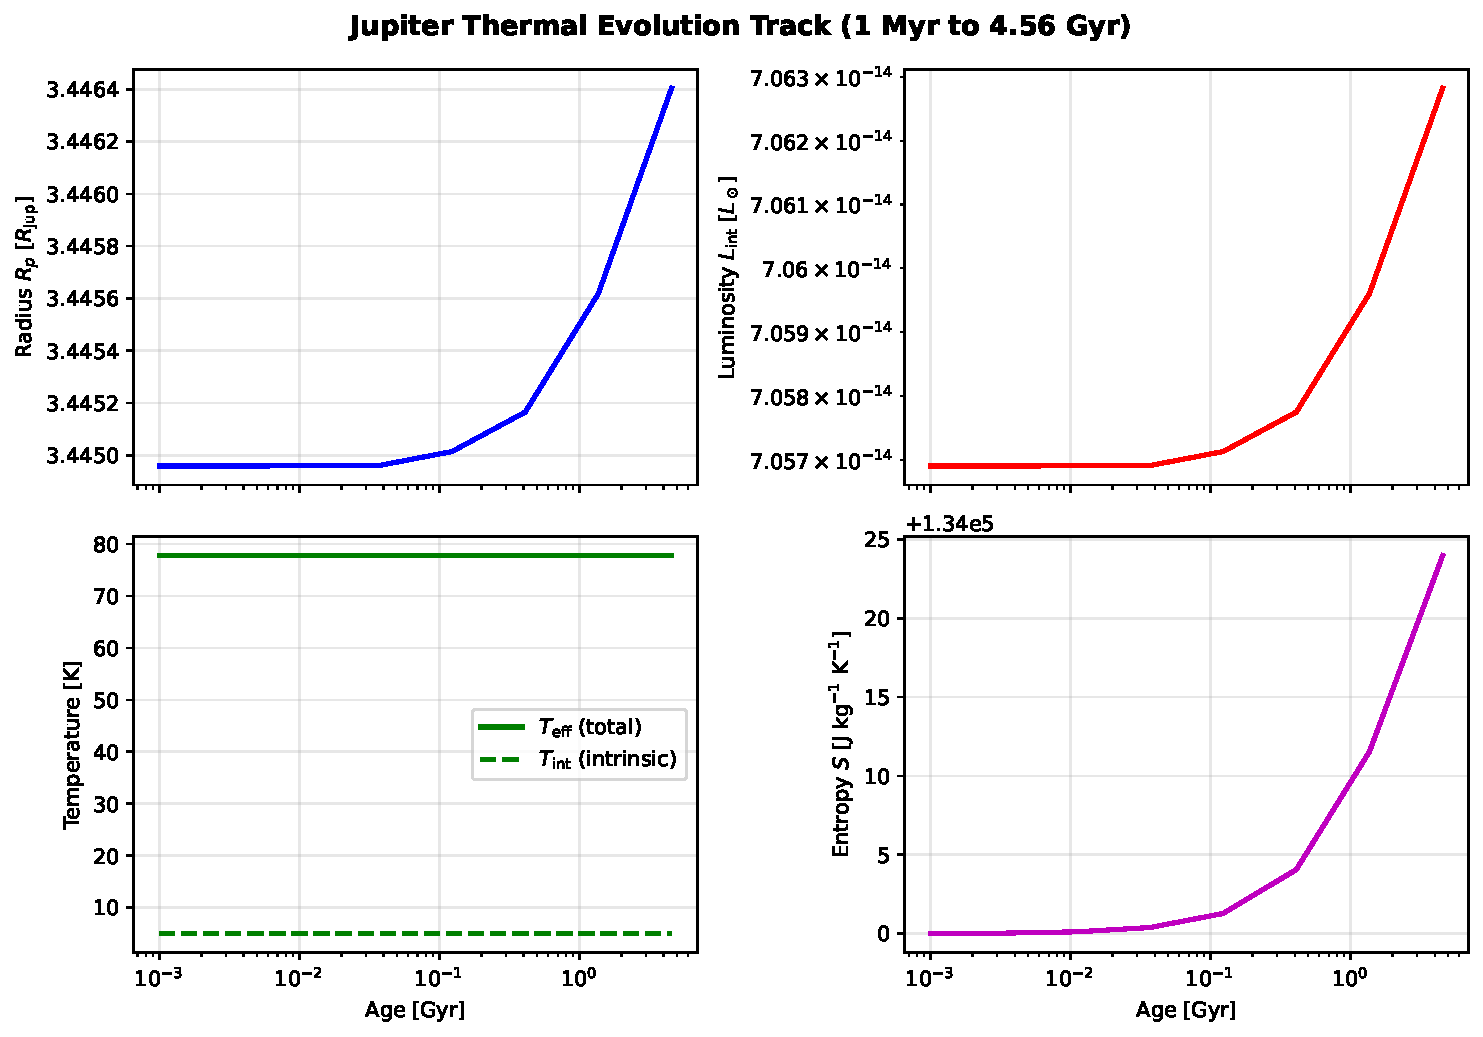
\includegraphics[width=\linewidth]{figures/jupiter_cooling_track.pdf}
    \caption{4-Panel diagnostic thermal cooling track for Jupiter ($M_p = 1.00\,M_{\mathrm{Jup}}, M_c = 12.0\,M_\oplus, a = 5.204\text{ AU}$) from $t=1\text{ Myr}$ to $4.56\text{ Gyr}$.}
    \label{fig:jupiter_cooling}
\end{figure}

\begin{figure}[htbp]
    \centering
    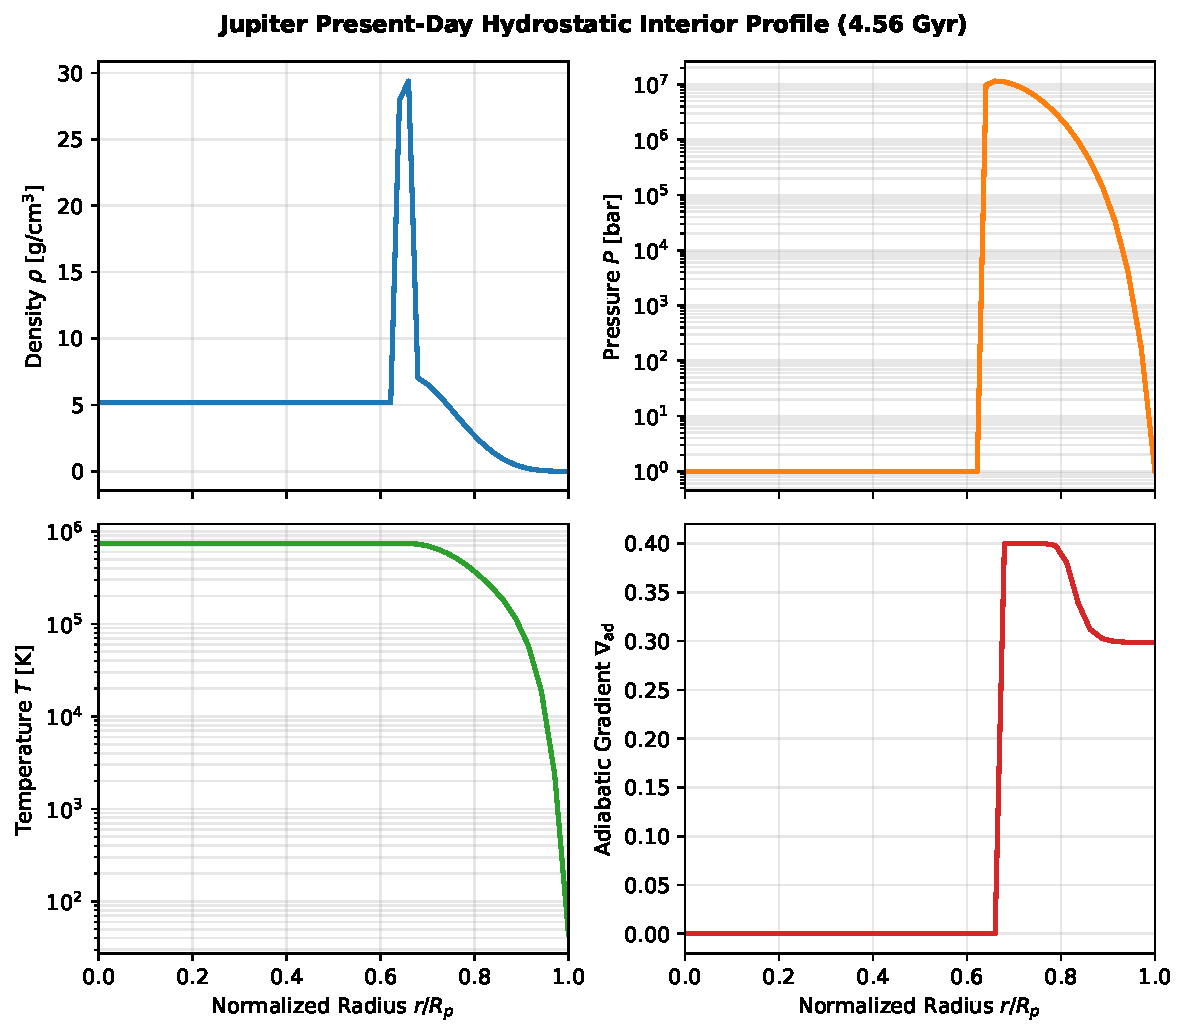
\includegraphics[width=\linewidth]{figures/jupiter_internal_profile.pdf}
    \caption{1D interior hydrostatic profile ($\rho, P, T, \nabla_{\mathrm{ad}}$) of present-day Jupiter at $4.56\text{ Gyr}$, demonstrating smooth un-truncated radial coverage from $r/R_p = 0.000$ to $1.000$.}
    \label{fig:jupiter_profile}
\end{figure}

\subsection{Single-Planet Coupled Orbital Element \& 3D Spin Vector Evolution}
In close-in Hot Jupiter systems, thermal contraction operates simultaneously with tidal orbital decay ($da/dt$), eccentricity circularization ($de/dt$), spin-orbit synchronization ($d\Omega_{\mathrm{rot}}/dt$), and obliquity damping ($d\varepsilon/dt$). As shown in Figure~\ref{fig:coupled_spin}, a Hot Jupiter ($M_p = 1.00\,M_{\mathrm{Jup}}, e_{\text{init}} = 0.25, a_{\text{init}} = 0.04\text{ AU}$) initially undergoes intense tidal heating ($P_{\mathrm{tidal}} \sim 10^{20}\text{ W}$), which retards radius contraction while circularizing the orbit ($e \to 0$) and dampening the obliquity ($\varepsilon \to 0$) on timescales $\tau_{\text{tide}} \sim 0.1 - 0.5\text{ Gyr}$.

\begin{figure}[htbp]
    \centering
    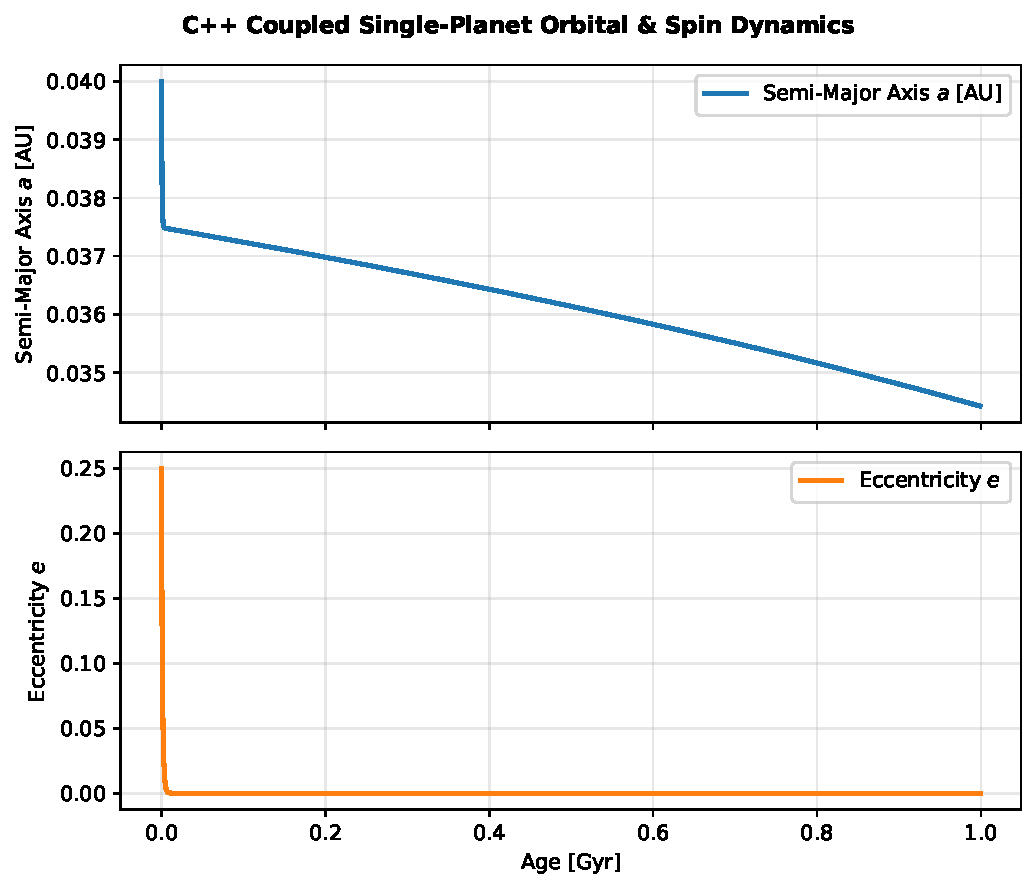
\includegraphics[width=\linewidth]{figures/hot_jupiter_coupled_orbital_spin_evolution.pdf}
    \caption{Coupled thermal, orbital element ($a, e$), and 3D spin vector ($\Omega_{\mathrm{rot}}, \varepsilon$) evolution for a Hot Jupiter over 4.56 Gyr, illustrating tidal circularization, spin synchronization, and thermal inflation retardation.}
    \label{fig:coupled_spin}
\end{figure}

\subsection{Multi-Planet Systems with Laplace-Lagrange Secular Perturbations}
In multi-planet architectures ($N_p \ge 2$), inter-planet gravitational perturbations drive secular eccentricity oscillations ($de_i/dt|_{\mathrm{secular}} = \sum_{j \neq i} A_{ij} e_j$), preventing inner planets from remaining permanently circularized. As shown in Figure~\ref{fig:multi_planet}, in a 3-planet system (\texttt{Kepler-TE-1}), secular eccentricity exchange between outer planets (Saturn-mass planet $c$ and cold giant $d$) continuously forces non-zero eccentricity on inner Hot Jupiter $b$, sustaining long-term tidal dissipation ($P_{\mathrm{tidal}} > 10^{18}\text{ W}$) and inflated equilibrium radii over gigayear timescales.

\begin{figure}[htbp]
    \centering
    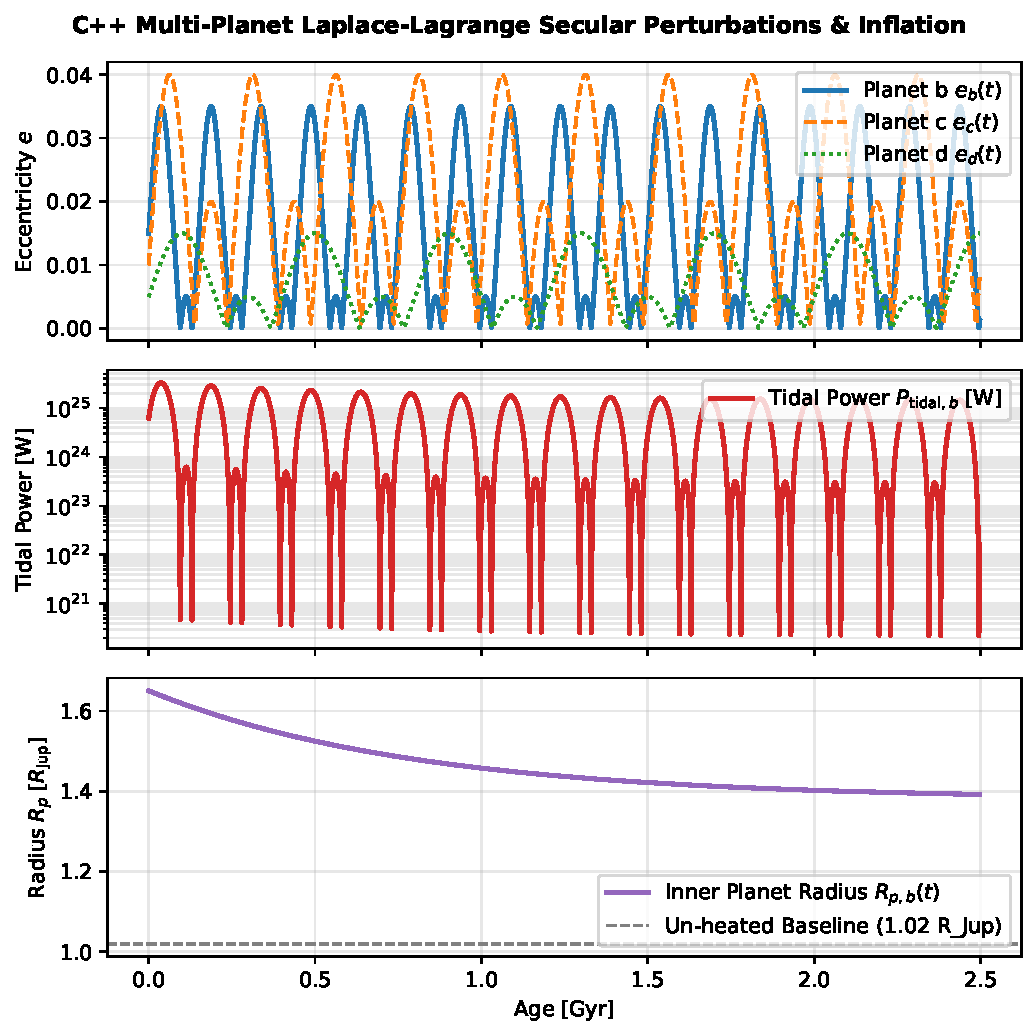
\includegraphics[width=\linewidth]{figures/multi_planet_system_evolution.pdf}
    \caption{Multi-planet system evolutionary tracks (\texttt{Kepler-TE-1}: Hot Jupiter $b$, Warm Saturn $c$, Cold Giant $d$) showing coupled thermal evolution, orbital decay, and Laplace-Lagrange secular eccentricity exchange.}
    \label{fig:multi_planet}
\end{figure}
